\documentclass{article}
\usepackage[utf8]{inputenc}

% Page setup
\usepackage[a4paper,landscape,margin=2cm]{geometry}

% Typography
\usepackage[scaled]{helvet}
\let\familydefault\sfdefault

\usepackage[usenames,svgnames]{xcolor}
\usepackage{tikz}
\usetikzlibrary{positioning,arrows}

\definecolor{colorbg}  {RGB}{199,212,104}
\definecolor{colortext}{RGB}{29,29,27}

\begin{document}
\pagestyle{empty}
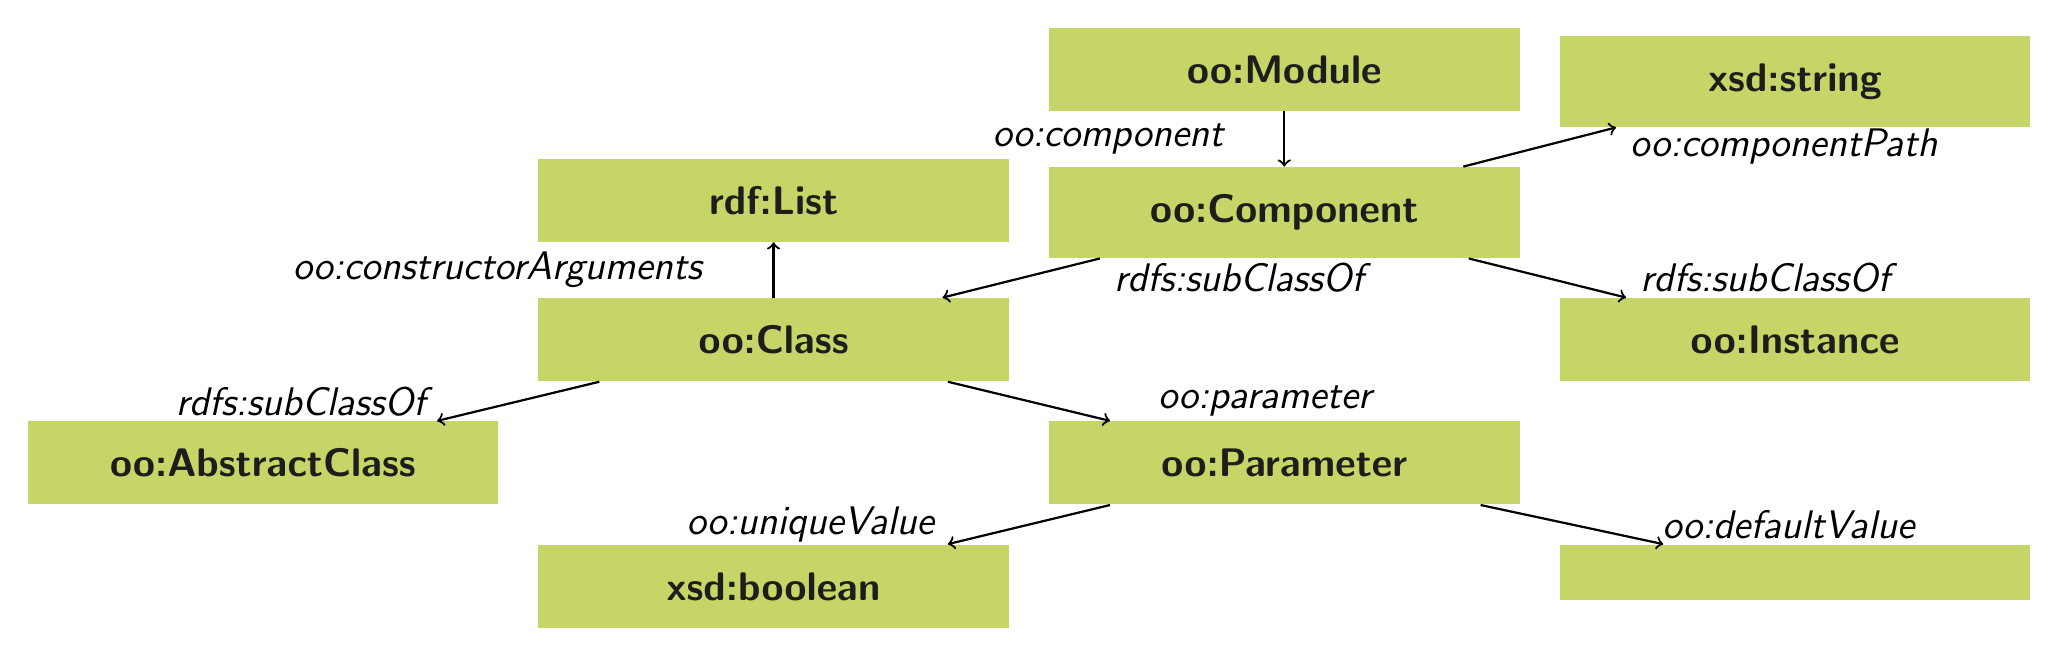
\begin{tikzpicture}[
    node distance = 2em, auto,
    font={\Large\itshape},
    concept/.style={text=colortext,font={\Large\bfseries},inner sep=10pt,align=center,rectangle,fill=colorbg,text width=15em},
    relation/.style={text width=12em},
]

    % Concepts
    \node[concept] (module)    {oo:Module};
    \node[concept, below=of module] (component) {oo:Component};
    
    \node[concept, below left=of component] (class) {oo:Class};
    \node[concept, below left=of class] (classAbstract) {oo:AbstractClass};
    \node[concept, above=of class] (args) {rdf:List};
    
    \node[concept, above right=of component]       (string)   {xsd:string};
    \node[concept, below right=of component] (instance) {oo:Instance};
    
    \node[concept, below right=of class] (parameter)     {oo:Parameter};
    \node[concept, below left=of parameter] (boolean)    {xsd:boolean};
    \node[concept, below right=of parameter] (blank)     {\ };
    
    % Concept relations
    \draw[->,thick,relation] (module) -- (component) node [left,midway,align=center] {oo:component};
    \draw[->,thick,relation] (component) -- (class) node [right,midway,align=right] {rdfs:subClassOf};
    \draw[->,thick,relation] (component) -- (instance) node [right,midway,align=right] {rdfs:subClassOf};
    \draw[->,thick,relation,text width=14em] (component) -- (string) node [right,midway,align=right] {oo:componentPath};
    
    \draw[->,thick,relation] (class) -- (classAbstract) node [left,midway,align=left] {rdfs:subClassOf};
    \draw[->,thick,relation] (class) -- (parameter) node [right,midway,align=right] {oo:parameter};
    \draw[->,thick,relation,text width=17em] (class) -- (args) node [left,midway,align=left] {oo:constructorArguments};
    
    \draw[->,thick,relation] (parameter) -- (blank) node [right,midway,align=right] {oo:defaultValue};
    \draw[->,thick,relation] (parameter) -- (boolean) node [left,midway,align=left] {oo:uniqueValue};

\end{tikzpicture}
\end{document}
